\section{Dokumentace skriptu pro pokročilé objekty}

\subsection{Vytváření pokročilých triggerů}
Nejdříve je provedeno naplnění tabulky daty. Ta jsou vytvořena, pokud možno, co nejrůznoroději tak,
aby byly pokryty všechny eventuální kombinace pokročilých dotazů.

Jelikož se projekt zabývá půjčovnou hudebních nosičů s různými alby o různých délkách skladeb,
bylo vhodné vytvořit \texttt{databázový trigger} nad počítáním celkové délky alba při známé délce jednotlivých skladeb. 
Tento trigger má název \texttt{auto\_album\_length\_trigger}, přičemž po přidání, 
aktualizaci, nebo odstranění skladby z alba deklaruje čtyři pomocné proměnné, které pomáhají s následnou úpravou celkového času.

Druhý a třetí trigger kontrolují správnost zadávání dat při manipulaci s výpůjčkou nosiče. Při přidávání,
nebo editaci dat v tabulce \texttt{CARRIER\_BORROW\_RECORDS} automaticky kontrolují validitu dat vrácení, 
resp. očekávaného vrácení a při chybném vstupu volají výjimku.
Dalším užitečným triggerem by mohla být kontrola jestli nově zadaný carrier collection neobsahuje nosič co už je půjčený.



\subsection{Optimalizace dotazů}
Princip optimalizace dotazů je v tomto projektu předveden na dvou případech. 
Dotaz zjišťující počet vypůjčených nosičů alb v jednotlivých měsících nejdříve proběhl standardně,
tedy prostým příkazem \texttt{SELECT} z tabulky \texttt{CARRIER\_BORROW\_RECORDS}. 
V takovém případě byla jeho cena 5 (obr. \ref{fig:pic1}). 
Následně byl přidán index přistupující ke sloupci data vypůjček téže tabulky. 
V takovém případě spadla jeho cena na hodnotu 3 (obr. \ref{fig:pic2}). 
Tento dotaz, vzhledem ke své minimálnosti, by bylo obtížné dále optimalizovat.

\begin{figure}[h]
    \centering
    \caption{\texttt{EXPLAIN PLAN} \textbf{před} optimalizací}
    \label{fig:pic1}

    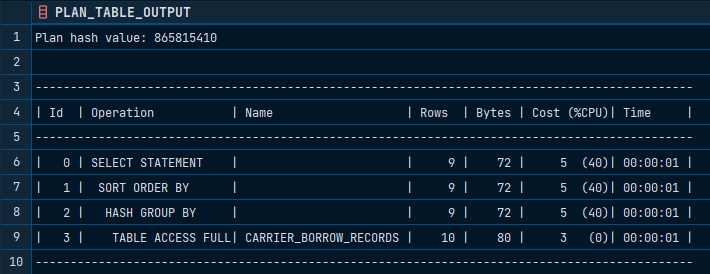
\includegraphics[scale=0.8]{1-1.png}
\end{figure}

\begin{figure}[h]
    \centering
    \caption{\texttt{EXPLAIN PLAN} \textbf{po} optimalizací}
    \label{fig:pic2}
    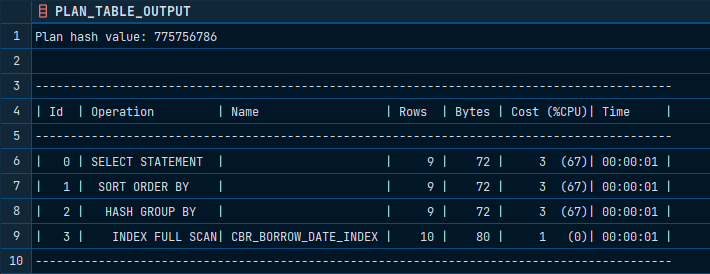
\includegraphics[scale=0.8]{1-2.png}
\end{figure}


\newpage
Druhá optimalizace je znázorněna na dotazu vypisujícím jména zákazníků, kteří si kdy vypůjčili album \textit{The best of Waterflame}. 
Po spojení čtyř tabulek je při standardní cestě  cena dotazu 12 (obr. \ref{fig:pic3}). 
Po vytvoření indexu do jmenného sloupce tabulky alb spadne cena dotazu na hodnotu 11 (obr. \ref{fig:pic4}). 
Tento výsledek by šel ještě dále vylepšit přidáním indexů do tabulky \texttt{CARRIER\_COLLECTION}, 
ale vzhledem k malému počtu záznamů by náročnost moc nevylepšilo.


\begin{figure}[h]
    \centering
    \caption{\texttt{EXPLAIN PLAN} \textbf{před} optimalizací}
    \label{fig:pic3}
    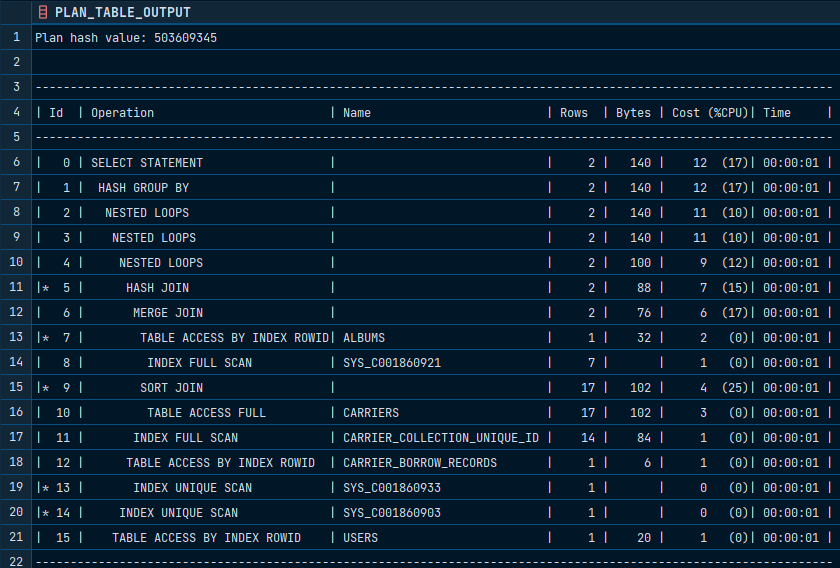
\includegraphics[scale=0.65]{2-1.png}
\end{figure}


\begin{figure}[h]
    \centering
    \caption{\texttt{EXPLAIN PLAN} \textbf{po} optimalizací}
    \label{fig:pic4}
    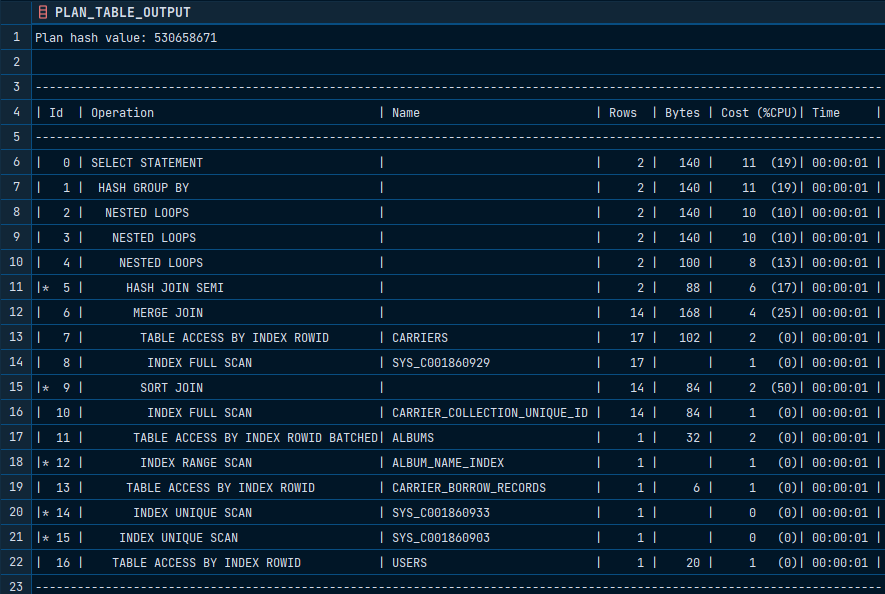
\includegraphics[scale=0.65]{2-2.png}
\end{figure}



\newpage
\subsection{Práva a materializovaný pohled}
Definice přístupových práv k databázovým objektům pro druhého člena týmu byly provedeny příkazy:

\medskip
\noindent
\texttt{GRANT~ALL~PRIVILEGES~ON~\dots~TO~\dots}

\medskip
\noindent
a to pro každý databázový objekt zvlášť. Řešitelům se bohužel nepodařilo tuto konstrukci minimalizovat. 

Pro demonstraci materializovaného pohledu \texttt{late\_returners} patřící prvnímu členu týmu, 
kde tabulky byly definované druhým členem týmu, byl vybrán dotaz na konkrétní osoby, které překračují výpůjční dobu. 
Toto bylo dosaženo spojením čtyř tabulek autora \texttt{xdousa00}. Pohled pak patří uživateli \texttt{xpospi0k} s příslušnými právy. 
Konkrétní \texttt{SELECT} následuje v kódu vzápětí,  přičemž jednoduše vybere všechny záznamy.
